Bibika está jogando o famoso jogo Navalha Batal. Para quem não conhece, o jogo é basicamente jogado entre duas pessoas onde existe um tabuleiro de tamanho NxN com algumas peças (que representam Bavios) de tamanhos 1xT e Tx1 previamente inseridas, onde o valor de T é inteiro positivo menor ou igual a N. Vale ressaltar que a sobreposição de peças não é possível.

Após posicionarem suas peças iniciais, cada jogador tem alguns minutos para analisar o tabuleiro e então devem calcular (ou chutar) a quantidade de peças 1xT e Tx1 que ainda podem ser inseridas de forma independente. \newline

Segue um exemplo de um tabuleiro 3x3 com 4 posições [(1,2), (2,3), (3,1) e (3,2)] previalmente preenchidas pelos jogadores.

\begin{figure}[h!]
\centering
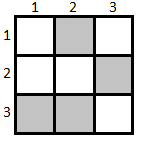
\includegraphics[scale=0.7]{tab_inicial.png}
\end{figure}

Nesse caso ainda é possível inserir nas células vazias 7 peças de tamanhos 1xT ou Tx1, todas ilustradas abaixo:

\begin{figure}[h!]
\centering
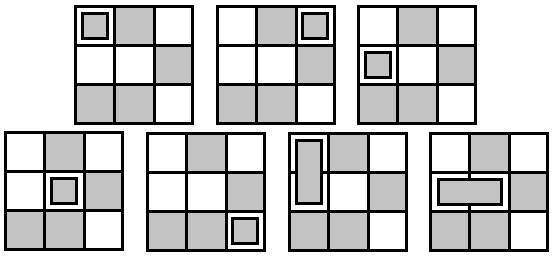
\includegraphics[scale=0.6]{pecas.png}
\end{figure}

Após jogarem com um tabuleiro de tamanho consideravelmente pequeno, Bibika gostaria de saber a resposta para tabuleiros maiores. Como é uma tarefa bastante complexa a olho nu, cabe a você ajudá-la!

\section*{Entrada}

A primeira linha contém dois inteiros $N$ e $Q$, sendo $N$ o tamanho do tabuleiro quadrado e $Q$ a quantidade de células distintas que estão previamente preenchidas.
As próximas $Q$ linhas possuem dois inteiros, $X_i$ e $Y_i$, indicando que a coordenada $X_i, Y_i$ do tabuleiro está preenchida.

\section*{Saída}

Exiba um único inteiro, a quantidade de bavios de tamanho $1xT$ ou $Tx1$ que ainda são possíveis de serem colocados de forma que fiquem totalmente inseridos no tabuleiro e não exista sobreposição com outros bavios. Como a quantidade pode ser muito grande, exiba a quantidade módulo $10^9+7$.

\section*{Restrições}

$1 \leq N \leq 10^6$
$0 \leq Q \leq 10^5$
$1 \leq X, Y \leq N$

\section*{Exemplos}
\exemplo